% ------------------------------------------------------------------------------
\subsection{Synchronisation}

% ▿▿▿▿▿▿▿▿▿▿▿▿▿▿▿▿▿▿▿▿▿▿▿▿▿▿▿▿▿▿▿▿▿▿▿▿▿▿▿▿▿▿▿▿▿▿▿▿▿▿▿▿▿▿▿▿▿▿▿▿▿▿▿▿▿▿▿▿▿▿▿▿▿▿▿▿▿▿
\begin{frame}
\tableofcontents[subsectionstyle=show/shaded/hide, subsubsectionstyle=hide, sectionstyle=show/hide]
\end{frame}
% ▵▵▵▵▵▵▵▵▵▵▵▵▵▵▵▵▵▵▵▵▵▵▵▵▵▵▵▵▵▵▵▵▵▵▵▵▵▵▵▵▵▵▵▵▵▵▵▵▵▵▵▵▵▵▵▵▵▵▵▵▵▵▵▵▵▵▵▵▵▵▵▵▵▵▵▵▵▵

% ▿▿▿▿▿▿▿▿▿▿▿▿▿▿▿▿▿▿▿▿▿▿▿▿▿▿▿▿▿▿▿▿▿▿▿▿▿▿▿▿▿▿▿▿▿▿▿▿▿▿▿▿▿▿▿▿▿▿▿▿▿▿▿▿▿▿▿▿▿▿▿▿▿▿▿▿▿▿
\begin{frame}
\frametitle{Introduction}

\begin{block}{Contexte}
\begin{itemize}
    \item Liaison réseau pas toujours accessible % Ouragan, tremblements de terre
    \item Plusieurs utilisateurs peuvent modifier la même donnée % Dans le cas où ils sont offline, ça va poser pb
\end{itemize}
\end{block}

\pause

\begin{alertblock}{Problématique}
\begin{itemize}
    \item Cohérence des données
    \item Conflits
\end{itemize}
\end{alertblock}

\end{frame}
% ▵▵▵▵▵▵▵▵▵▵▵▵▵▵▵▵▵▵▵▵▵▵▵▵▵▵▵▵▵▵▵▵▵▵▵▵▵▵▵▵▵▵▵▵▵▵▵▵▵▵▵▵▵▵▵▵▵▵▵▵▵▵▵▵▵▵▵▵▵▵▵▵▵▵▵▵▵▵

% ▿▿▿▿▿▿▿▿▿▿▿▿▿▿▿▿▿▿▿▿▿▿▿▿▿▿▿▿▿▿▿▿▿▿▿▿▿▿▿▿▿▿▿▿▿▿▿▿▿▿▿▿▿▿▿▿▿▿▿▿▿▿▿▿▿▿▿▿▿▿▿▿▿▿▿▿▿▿
\begin{frame}
\frametitle{Introduction}

\begin{exampleblock}{Idée}
\begin{itemize}
    \item Gérer deux modes~: Connecté (synchrone), Hors-ligne (asynchrone)
    \item Logger tout ajout ou modification (avec horodatage)
    \item S'en servir pour la fusion
\end{itemize}
\end{exampleblock}

\end{frame} % Fin de la frame [Introduction]
% ▵▵▵▵▵▵▵▵▵▵▵▵▵▵▵▵▵▵▵▵▵▵▵▵▵▵▵▵▵▵▵▵▵▵▵▵▵▵▵▵▵▵▵▵▵▵▵▵▵▵▵▵▵▵▵▵▵▵▵▵▵▵▵▵▵▵▵▵▵▵▵▵▵▵▵▵▵▵

% ▿▿▿▿▿▿▿▿▿▿▿▿▿▿▿▿▿▿▿▿▿▿▿▿▿▿▿▿▿▿▿▿▿▿▿▿▿▿▿▿▿▿▿▿▿▿▿▿▿▿▿▿▿▿▿▿▿▿▿▿▿▿▿▿▿▿▿▿▿▿▿▿▿▿▿▿▿▿
\begin{frame}
\frametitle{Modes de connexion}
\begin{figure}[htbp]
    \centering
    \scalebox{0.5}{
	    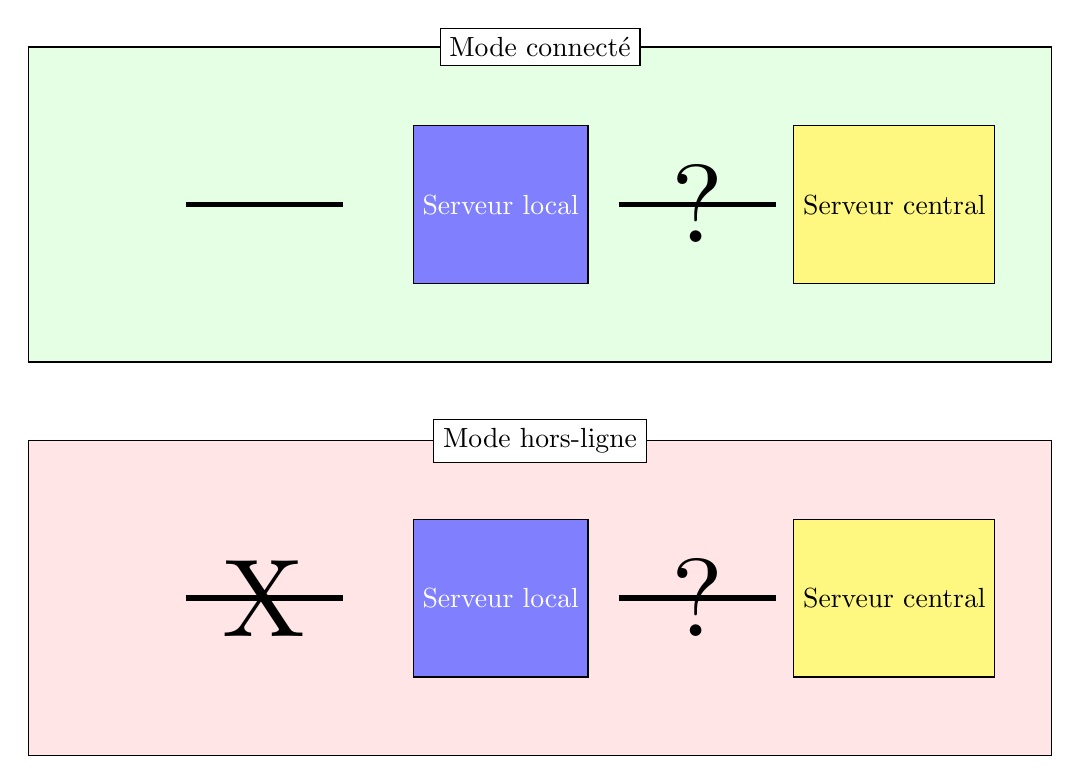
\begin{tikzpicture}
	        % Styles :
		    \tikzstyle{titre}=[rectangle,draw,fill=white,text=black]
		    \tikzstyle{symbole}=[rectangle,text=black, scale=4]
		    \tikzstyle{serveurloc}=[rectangle,draw,fill=blue!50,text=white, minimum height=2cm]
		    \tikzstyle{serveurcen}=[rectangle,draw,fill=yellow!50,text=black, minimum height=2cm]
	        % #### CADRE ROUGE :
		    % Fond :
		    \draw[fill=red!10] (0,0) rectangle (13, 4);
		    % Titres :
		    \node[titre] at (6.50,4.00) {Mode hors-ligne};
		    % Serveurs :
		    \node[serveurloc] at (6.00,2) {Serveur local};
		    \node[serveurcen] at (11.00,2) {Serveur central};
		    \node[symbole] at (8.50,2) {?};
		    \node[symbole] at (3.00,2) {X};
		    % Traits :
		    \draw[line width=2pt] (2, 2) -- (4, 2);
		    \draw[line width=2pt] (7.5, 2) -- (9.5, 2);
		    % Utilisateurs :
		    \umlactor[x=1.00, y=2.00]{Utilisateur}
		    % #### CADRE VERT :
		    % Fond :
		    \draw[fill=green!10] (0,5) rectangle (13, 9);
		    % Titres :
		    \node[titre] at (6.50,9.00) {Mode connecté};
		    % Serveurs :
		    \node[serveurloc] at (6.00,7) {Serveur local};
		    \node[serveurcen] at (11.00,7) {Serveur central};
		    \node[symbole] at (8.50, 7) {?};
		    % Traits :
		    \draw[line width=2pt] (2, 7) -- (4, 7);
		    \draw[line width=2pt] (7.5, 7) -- (9.5, 7);
		    % Utilisateurs :
		    \umlactor[x=1.00, y=7]{Utilisateur}
	    \end{tikzpicture}
    }
	\caption{Topologie des modes connecté et hors-ligne}
	\label{explicationcodeco}
\end{figure}
\end{frame} % Fin de la frame [Synchronisation]
% ▵▵▵▵▵▵▵▵▵▵▵▵▵▵▵▵▵▵▵▵▵▵▵▵▵▵▵▵▵▵▵▵▵▵▵▵▵▵▵▵▵▵▵▵▵▵▵▵▵▵▵▵▵▵▵▵▵▵▵▵▵▵▵▵▵▵▵▵▵▵▵▵▵▵▵▵▵▵

% ▿▿▿▿▿▿▿▿▿▿▿▿▿▿▿▿▿▿▿▿▿▿▿▿▿▿▿▿▿▿▿▿▿▿▿▿▿▿▿▿▿▿▿▿▿▿▿▿▿▿▿▿▿▿▿▿▿▿▿▿▿▿▿▿▿▿▿▿▿▿▿▿▿▿▿▿▿▿
\begin{frame}
\frametitle{Ajout / Modification de donnée}

En simplifié :

\begin{block}{Mode hors-ligne}
\begin{enumerate}
%\setcounter{enumi}{}
    \item Demande d'ajout/modification de l'utilisateur
\end{enumerate}
\vspace{-1em}
\hspace*{.05\linewidth}\begin{minipage}{.9\linewidth}
\begin{exampleblock}{Mode connecté uniquement}
\begin{enumerate}
    \setcounter{enumi}{1}
    \item Demande de permission au serveur
    \item Envoi de l'ajout/modification
    \item Attente de confirmation
\end{enumerate}
\end{exampleblock}
\end{minipage}
\begin{enumerate}
\setcounter{enumi}{4}
    \item (Ssi première \emph{modification} :) \textbf{log} de la donnée originelle
    \item Application des changements en local
    \item \textbf{Log} des détails du changement
\end{enumerate}
\end{block}


\end{frame} % Fin de la frame [Ajout / Modification en mode connecté]
% ▵▵▵▵▵▵▵▵▵▵▵▵▵▵▵▵▵▵▵▵▵▵▵▵▵▵▵▵▵▵▵▵▵▵▵▵▵▵▵▵▵▵▵▵▵▵▵▵▵▵▵▵▵▵▵▵▵▵▵▵▵▵▵▵▵▵▵▵▵▵▵▵▵▵▵▵▵▵

% ▿▿▿▿▿▿▿▿▿▿▿▿▿▿▿▿▿▿▿▿▿▿▿▿▿▿▿▿▿▿▿▿▿▿▿▿▿▿▿▿▿▿▿▿▿▿▿▿▿▿▿▿▿▿▿▿▿▿▿▿▿▿▿▿▿▿▿▿▿▿▿▿▿▿▿▿▿▿
\begin{frame}
\frametitle{Synchronisation}

\begin{block}{Étapes}
\begin{enumerate}
    %\setcounter{enumi}{}
    \item Envoi de la date courrante au serveur % Pour pouvoir calculer les éventuels écarts entre la date client et la date serveur
    \item Récupération des logs ultérieurs à la dernière synchronisation
\end{enumerate}
\vspace{-1em}
\hspace*{.05\linewidth}\begin{minipage}{.9\linewidth}
    \begin{block}{Pour chaque donnée modifiée localement :}
    \begin{enumerate}
    \setcounter{enumi}{2}
        \item Vérification des droits
        \item Si conflit : Choix de l'utilisateur entre la donnée locale et la serveur (en fonction de l'originale)
    \end{enumerate}
    \end{block}
\end{minipage}
\begin{enumerate}
\setcounter{enumi}{4}
    \item Application des changements en local
    \item Génération d'\textbf{un} log global des modifications
    \item Envoi au serveur
    \item Attente de confirmation
    \item MAJ de la date de la dernière synchronisation
\end{enumerate}
\end{block} 

\end{frame} % Fin de la frame [Synchronisation]
% ▵▵▵▵▵▵▵▵▵▵▵▵▵▵▵▵▵▵▵▵▵▵▵▵▵▵▵▵▵▵▵▵▵▵▵▵▵▵▵▵▵▵▵▵▵▵▵▵▵▵▵▵▵▵▵▵▵▵▵▵▵▵▵▵▵▵▵▵▵▵▵▵▵▵▵▵▵▵

% ▿▿▿▿▿▿▿▿▿▿▿▿▿▿▿▿▿▿▿▿▿▿▿▿▿▿▿▿▿▿▿▿▿▿▿▿▿▿▿▿▿▿▿▿▿▿▿▿▿▿▿▿▿▿▿▿▿▿▿▿▿▿▿▿▿▿▿▿▿▿▿▿▿▿▿▿▿▿
\begin{frame}
\frametitle{Trafic réseau}

\begin{block}{Communications restreintes}
    \begin{itemize}
        \item GSM ou Satellitaire
        \item Débits faibles
    \end{itemize}
\end{block}

\begin{exampleblock}{Contre-mesures}
\begin{itemize}
    \item Choix des éléments synchronisables
    \item Log unique pour l'ajout/modification (synchronisation)
\end{itemize}
\end{exampleblock}

\end{frame} % Fin de la frame [Gestion du trafic réseau]
% ▵▵▵▵▵▵▵▵▵▵▵▵▵▵▵▵▵▵▵▵▵▵▵▵▵▵▵▵▵▵▵▵▵▵▵▵▵▵▵▵▵▵▵▵▵▵▵▵▵▵▵▵▵▵▵▵▵▵▵▵▵▵▵▵▵▵▵▵▵▵▵▵▵▵▵▵▵▵

% Fin de la sous-section [Synchronisation]
% ------------------------------------------------------------------------------

% ▿▿▿▿▿▿▿▿▿▿▿▿▿▿▿▿▿▿▿▿▿▿▿▿▿▿▿▿▿▿▿▿▿▿▿▿▿▿▿▿▿▿▿▿▿▿▿▿▿▿▿▿▿▿▿▿▿▿▿▿▿▿▿▿▿▿▿▿▿▿▿▿▿▿▿▿▿▿
% ▵▵▵▵▵▵▵▵▵▵▵▵▵▵▵▵▵▵▵▵▵▵▵▵▵▵▵▵▵▵▵▵▵▵▵▵▵▵▵▵▵▵▵▵▵▵▵▵▵▵▵▵▵▵▵▵▵▵▵▵▵▵▵▵▵▵▵▵▵▵▵▵▵▵▵▵▵▵
